\section{Methods}
\label{sec:methods}

We estimate and analyze cell class-specific connectivity functions using models trained on murine brain viral tracing experiments.
This section describes the data used to generate the model, the model itself, the evaluation of the model against its alternatives, and the use of the model in creation of the connectivity estimate matrices.
It also includes background on the non-negative matrix factorization method used for decomposing the wild type connectivity matrix into latent factors.
Additional information about our data and methods are given in Supplemental Sections \ref{supp_sec:data} and \ref{supp_sec:methods}, respectively.

\newpage
\begin{figure}[H]
\subfloat[]{
\label{fig:mouse}
    
\includegraphics[width=0.3\textwidth]{figs/figure1a.png}}
\subfloat[]{
\label{fig:injproj}
    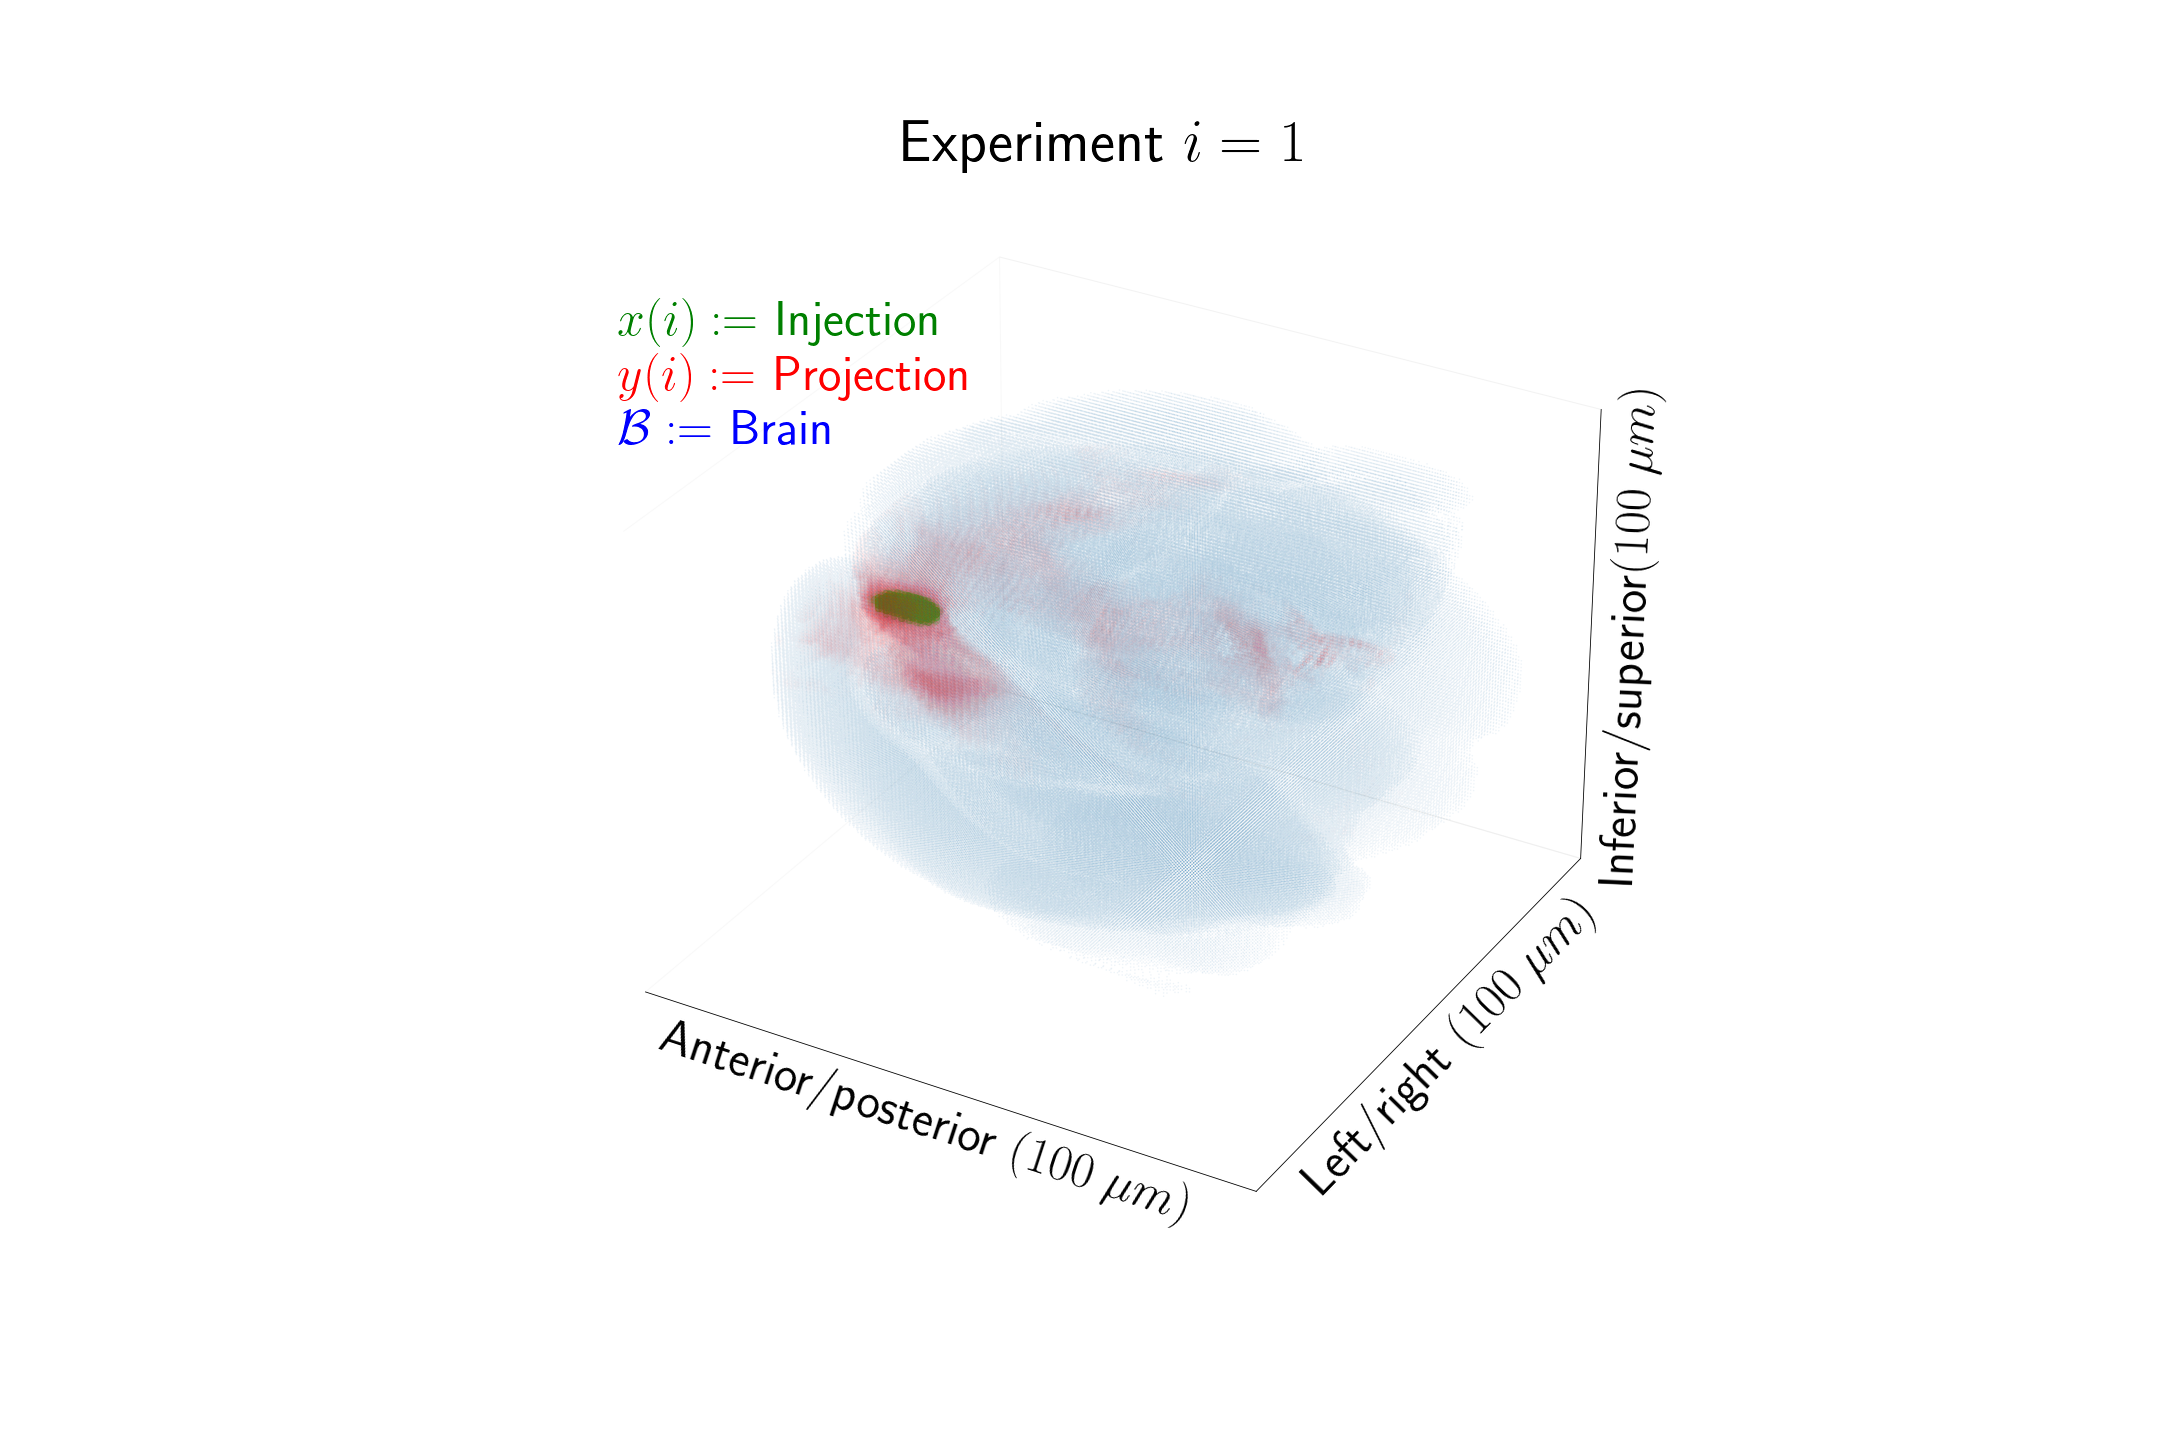
\includegraphics[width=0.4\textwidth]{figs/inj_proj_figure_v2.png}}
\subfloat[]{
\label{fig:segment}
    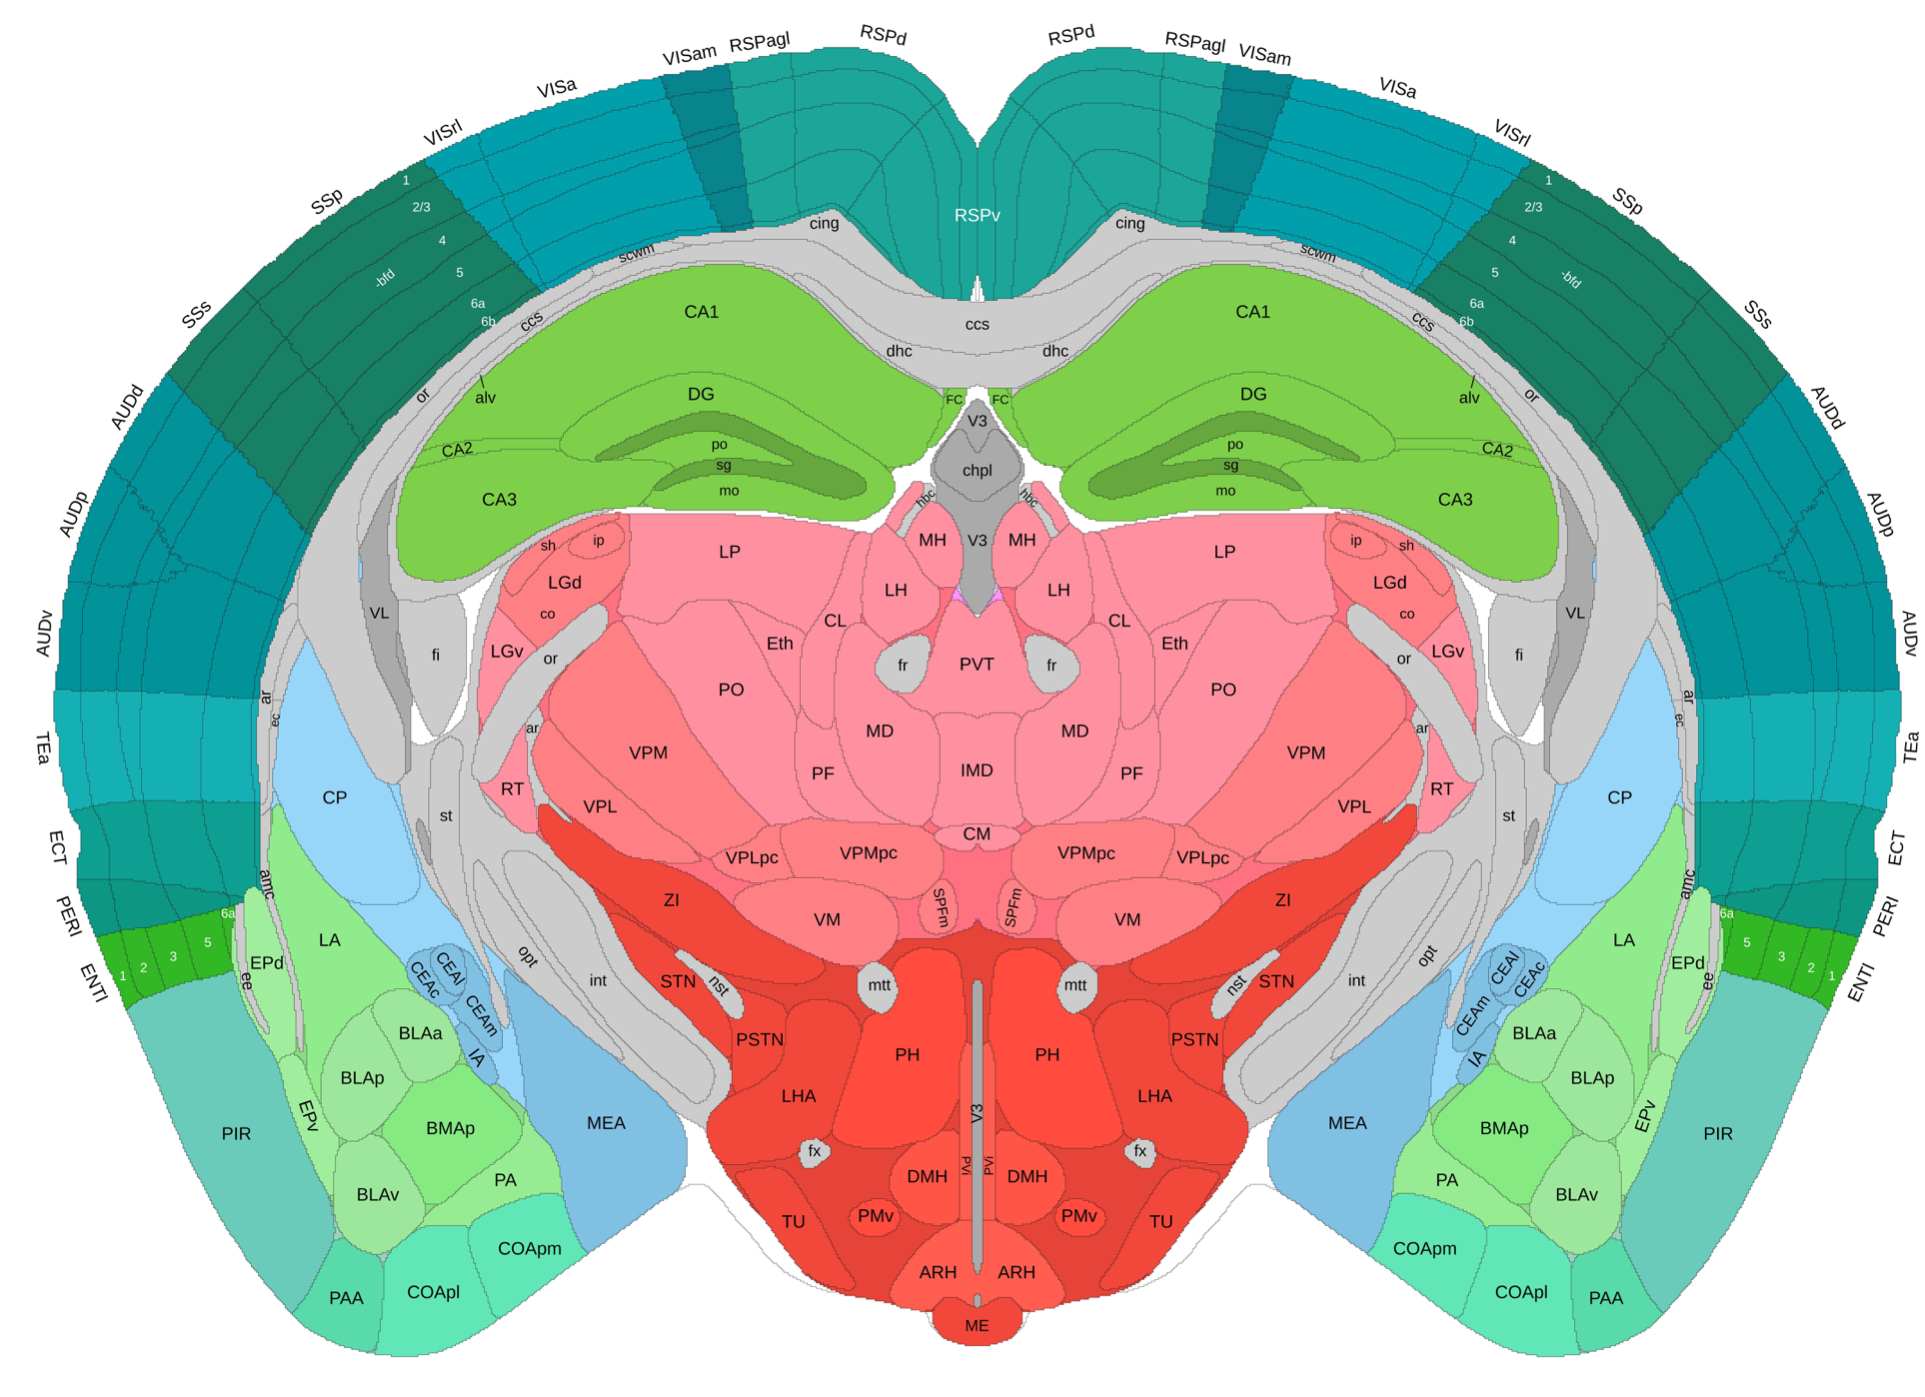
\includegraphics[width=0.3\textwidth]{figs/fig1c.png}}
    \newline
 \subfloat[]{
 \label{fig:ontology}
    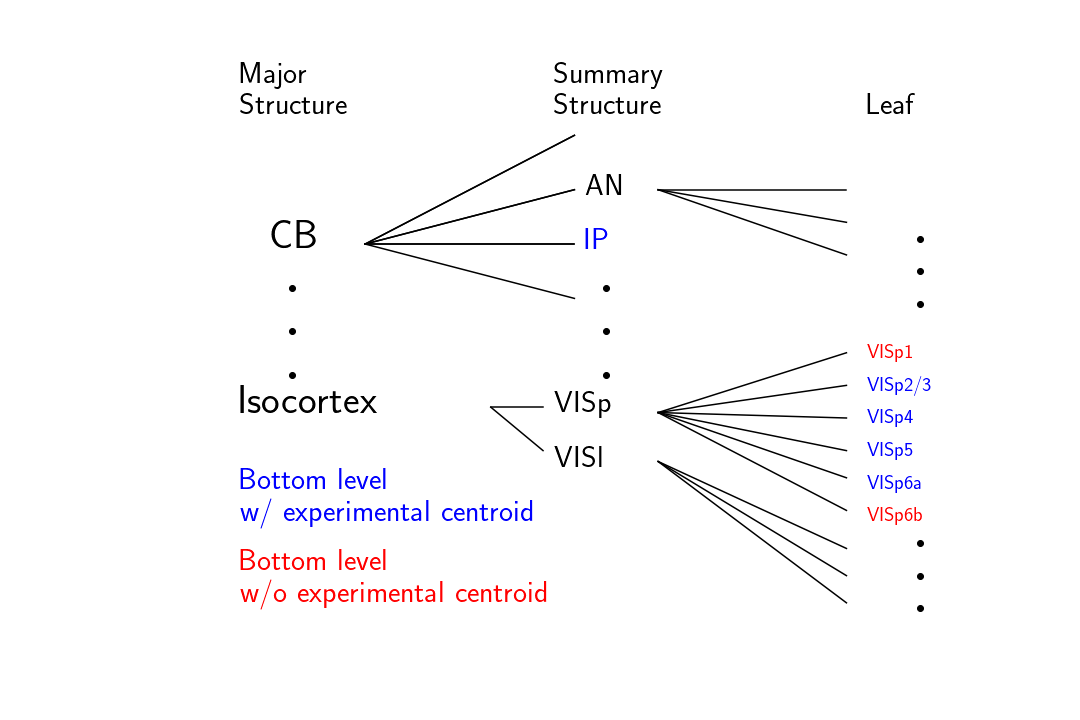
\includegraphics[width=0.35\textwidth]{figs/ontologyfigure.png}}
\subfloat[]{
 \label{fig:top}
    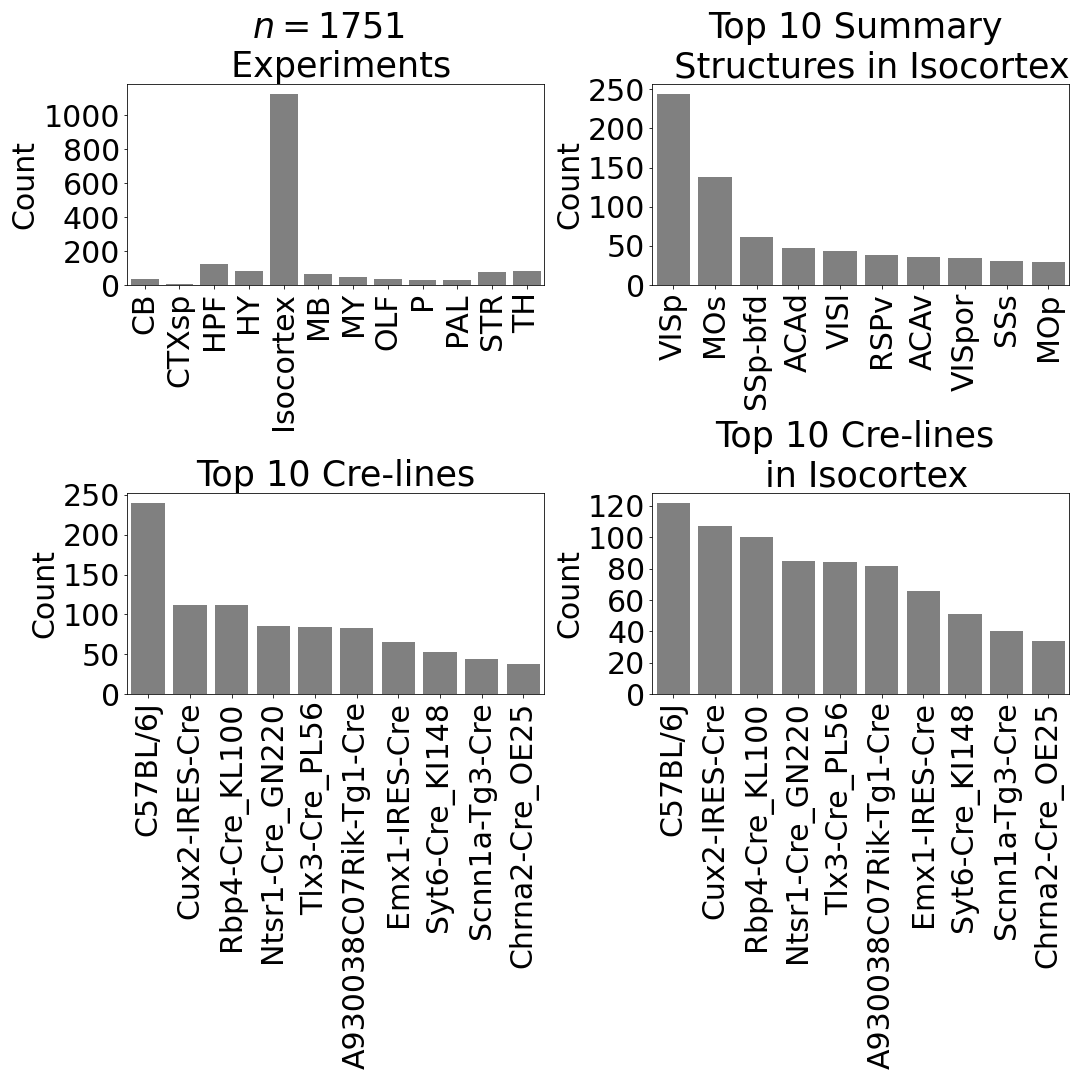
\includegraphics[width=0.35\textwidth]{figs/datasummary.png}}
\subfloat[]{
 \label{fig:combos}
    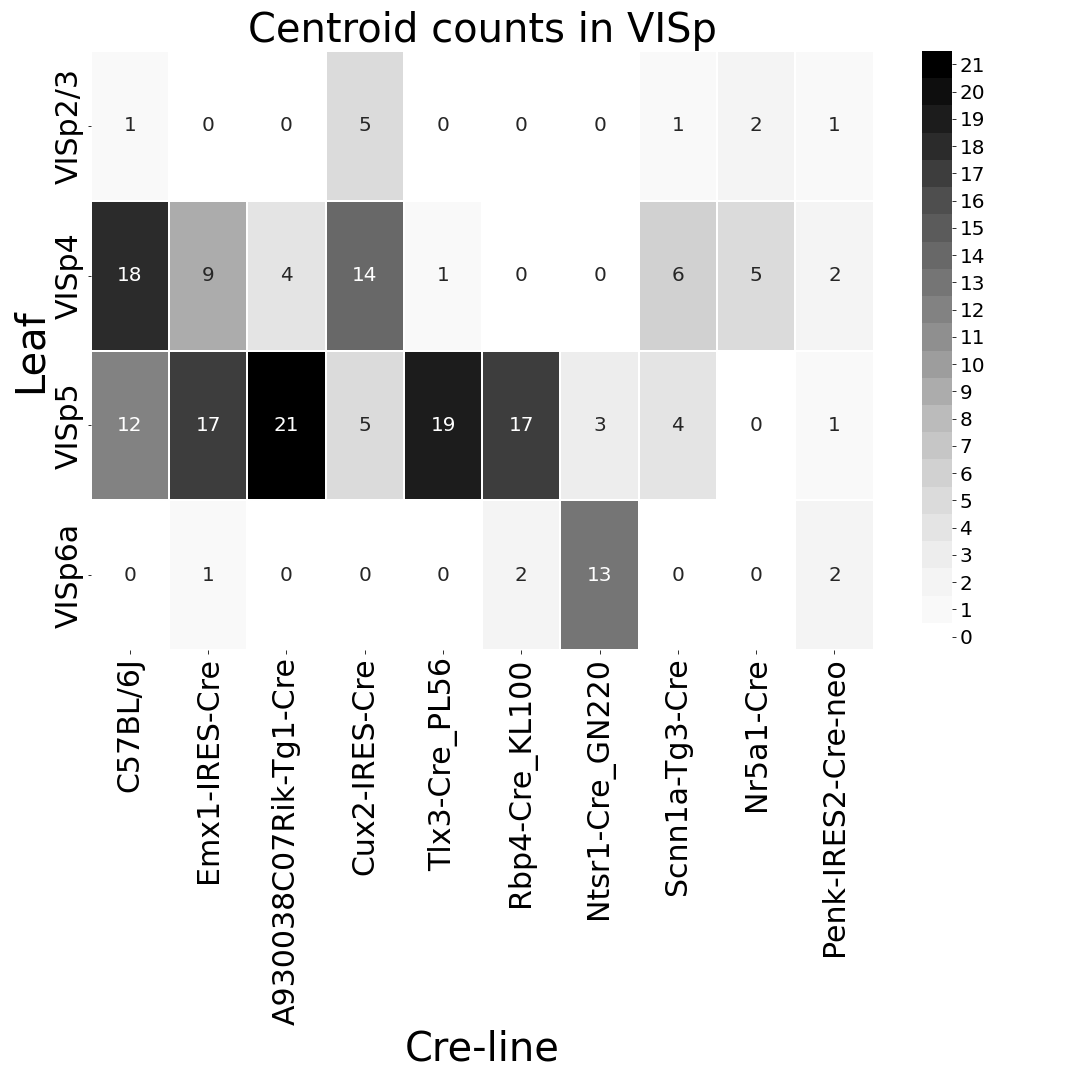
\includegraphics[width=0.35\textwidth]{figs/visp_counts.png}}   
    \caption{Experimental setting.  \ref{fig:mouse}  For each experiment, a Cre-dependent eGFP-expressing transgene casette is transduced by stereotaxic injection into a Cre-driver mouse, followed by serial two-photon tomography imaging.
    \ref{fig:injproj} An example of the segmentation of projection (targets) and injection (source) for a single experiment. Within each brain (blue), injection (green) and projection (red) areas are determined via histological analysis and alignment to the Allen Common Coordinate Framework (CCF).
    \ref{fig:segment} Brain region parcellations within a coronal plane of CCFv3. \ref{fig:ontology} Explanation of nested structural ontology highlighting various levels of CCFv3 structure ontology.
    Lowest-level (leaf) structures are colored in blue, and structures without an injection centroid are colored in red.
    \ref{fig:top}  Abundances of tracer experiments by Cre-line and region of injection. \ref{fig:combos}  Co-occurrence of layer-specific centroids and Cre-lines within VISp.}
    \label{fig:data}
\end{figure}

\newpage

\subsection{Data}

Our dataset $\mathcal D$ consists of $n=1751$ publicly available murine brain viral tracing experiments from the Allen Mouse Brain Connectivity Atlas.
Figure \ref{fig:mouse} summarizes the experimental process used to generate this data.
In each experiment, a mouse is injected with an adeno-associated virus (AAV) encoding green fluorescent protein (GFP) into a single location in the brain.
Location of fluorescence is mediated by the location of the injection, the characteristics of the transgene, and the genotype of the mouse.
In particular, Cre-driver or, equivalently, Cre-line mice are engineered to express Cre under the control of a specific and single gene promoter.
This localizes expression of Cre to regions with certain transcriptomic cell-types signatures.
In such Cre-driver mice, we used a double-inverted floxed AAV to produce eGFP fluorescence that depends on Cre expression in infected cells.
To account for the complex cell-type targeting induced by a particular combination of Cre-driver genotype and GFP promoter, we refer to the combinations of cell-types targeted by a particular combination of AAV and Cre-driver mice as cell-classes.
For example, we include experiments from Cre-driver lines that selectively label cell classes located in distinct cortical layers or other nuclei across the whole brain.
For injections in the wild type mice, we used the Synapsin I promoter \citep{Kugler2003-gz, Jackson2016-bw}.
For injections into Cre mice, we used the CAG promoter with a Flex cassette for Cre-mediated recombination control \citep{Saunders2012-xt}.
Additional details on are given in \citet{Harris2019-mr}.
%By our definition, wild type mice transduced with constitutitively active GFP promoters induce fluorescence of a particularly broad cell class.

For each experiment, the fluorescent signal imaged after injection is aligned into the Allen Common Coordinate Framework (CCF) v3, a three-dimensional average template brain that is fully annotated with regional parcellations \cite{Wang2020-po}.
The whole brain imaging and registration procedures described in detail in \citet{Oh2014-kh, Kuan2015-zz} produce quantitative metrics of fluorescence discretized at the $100 \; \mu$m \textbf{voxel} level. 
Given an experiment, this image was histologically segmented by an analyst into \textit{injection} and \textit{projection} areas corresponding to areas containing somas, dendrites and axons or exclusively axons of the transfected neurons.
An example of a single experiment rendered in 3D is given in Figure \ref{fig:injproj}.
Given an experiment $i$, we represent injections and projections as functions $x(i),y(i) : \mathcal B \to \mathbb R_{\geq 0}$, where $\mathcal B \subset [1:132] \times [1:80] \times [1:104]$ corresponds to the subset of the $(1.32 \times 0.8 \times 1.04)$ cm rectangular space occupied by the standard voxelized mouse brain.
We also calculate injection centroids $c(i) \in \mathbb R^3$ and regionalized projections $y_{\mathcal T} (i) \in \mathbb R^{T} $ given by the sum of $y(i)$ in each region.
A description of these steps is in Supplemental Section \ref{supp_sec:dp}.

Our goal is the estimation of \textbf{regionalized connectivity} from one region to another.
A visual depiction of this region parcellation for a two-dimensional slice of the brain is given in Figure \ref{fig:segment}.
All structures annotated in the CCF belong to a hierarchically ordered ontology, with different areas of the brain are parcellated to differing finer depths within a hierarchical tree.
We denote the main levels of interest as major structures, summary structures, and layers.
Not every summary structure has a layer decomposition within this ontology, so we typically consider the finest possible regionalization - for example, layer within the cortex, and summary structure within the thalymus, and denote these structures as leafs.
As indicated in Figure \ref{fig:ontology}, the dataset used to generate the connectivity model reported in this paper contains certain combinations of region and cell class frequently, and others not at all.
A summary of the most frequently assayed cell classes and structures is given in Figures \ref{fig:top} and \ref{fig:combos}.
Since users of the connectivity matrices may be interested in particular combinations, or interested in the amount of data used to generate a particular connectivity estimate, we present this information about all experiments in Supplemental Section \ref*{supp_sec:data}.

\newpage

\subsection{Modeling Regionalized Connectivity}
\label{sec:modelling}

We define voxelized cell-class specific connectivity $f:  \mathcal V \times \mathcal B \times \mathbb \mathcal \to \mathbb R_{\geq 0}$ as giving the voxelized connectivity strength of a particular cell class from a source voxel to a target voxel.
In contrast to \citet{Knox2019-ot}, which only uses wild type C57BL/6J mice, our dataset has experiments targeting $|\mathcal V| = 114$ different combinations of Cre-driver mice and Cre-regulated AAV transgenes jointly denoted as $\mathcal V := \{v\}$.
As in \citet{Knox2019-ot}, we ultimately estimate an integrated regionalized connectivity defined with respect to a set of $S = 564$ source leafs $\mathcal S := \{ s\} $ and $T = 1123$ target leafs $\mathcal T := \{ t \}$, of which $1123 - 564  = 559$ are contralateral.
That is, we define
\begin{align*}
&\text{\textit {regionalized connectivity strength} } \mathcal C : \mathcal V \times \mathcal S \times \mathcal T \to \mathbb R_{\geq 0}  \text{ with } \mathcal C(v,s,t) = \sum_{l_{j} \in s} \sum_{l_{j'} \in  t} f(v,l_{j},l_{j'}), \\
&\text{\textit {normalized regionalized connectivity strength} } \mathcal C^N : \mathcal V \times \mathcal S \times \mathcal T \to \mathbb R_{\geq 0}  \text{ with } \mathcal C^N(v,s,t) = \frac{1}{|s|} \mathcal C(v,l_{j},l_{j'}), \\
&\text{\textit {normalized regionalized projection density} } \mathcal C^D : \mathcal V \times \mathcal S \times \mathcal T \to \mathbb R_{\geq 0} \text{ with } \mathcal C^D(v,s,t) = \frac{1}{| s | | t|}\mathcal C(v,l_{j},l_{j'})
\end{align*}
where $l_j$ and $l_{j'}$ are the locations of source and target voxels, and $|s|$ and $|v|$ are defined to be the number of voxels in the source and target structure, respectively.
Since the normalized strength and densities are computable from the strength via a fixed normalization, our main statistical goal is to estimate $\mathcal C (v,s,t) $ for all $v, s$ and $t$.% and density are
In other words, we want to estimate matrices $\mathcal C_v \in \mathbb R_{\geq 0}^{S \times T}$.
We call this estimator $\widehat { \mathcal C } $.

Construction of such an estimator raises the questions of what data to use for estimating which connectivity, how to featurize the dataset, what statistical estimator to use, and how to reconstruct the connectivity using the chosen estimator.
We represent these considerations as 
\begin{align}
\label{eq:estimator}
\widehat { \mathcal C }(v,s,t) = f^* (\widehat f (f_*( \mathcal D(v,s))).
\end{align}
This makes explicit the data featurization $f_{*}$, statistical estimator $\widehat f$, and any potential subsequent transformation $f^*$ such as summing over the source and target regions.
Denoting $ \mathcal D$ as a function of $v$ and $s$ reflects that we consider using different data to estimate connectivities for different cell-classes and source regions.
Table \ref{tab:estimators} reviews estimators used for this data-type used in previous work, as well as our two main extensions: the Cre-NW and \textbf{Expected Loss} (EL) models.
The main differences in our data featurization from \citep{Knox2019-ot} are that we regionalize our data at the leaf level where available so that it layer-specific behavior is visible, and normalize our data by projection signal in order to account for differences between cell class.
Additional model selection results are given in Supplemental Section \ref{supp_sec:model-evaluation} for alternative normalization strategies, and more detail on estimation is given in Supplemental Section \ref{supp_sec:estimators}.

\begin{table}[H]
    \centering
    \begin{tabular}{c|c|c|c|c|}
        Name & $f^*$ & $\widehat f$&  $ f_*$ & $\mathcal D(v,s)$ \\
        \hline
        NNLS \citep{Oh2014-kh} & $\widehat f (1_s)$ & \nnls(X,Y) & $X= x_{\mathcal S},Y = y_{\mathcal T}$ & $ I_m / I_m$ \\
        NW \citep{Knox2019-ot} &$ \sum_{l_s \in s} \widehat f (l_s)$ & \nw(X,Y)  & $X = l_s, Y = y_{\mathcal T}$ & $I_m /I_m$ \\
        Cre-NW& $\sum_{l_s \in s} \widehat f(l_s)$ & \nw(X,Y) & $X= l_s, Y = y_{\mathcal T}$  &$ (I_l \cap I_v) / I_m$ \\
        Expected Loss (EL) & $\sum_{l_s \in s} \widehat f (s)$ & $\el(X,Y,v)$ & $X= l_s, Y = y_{\mathcal T}, v$  &$I_l / I_m$
    \end{tabular}
    \caption{Estimation of $\mathcal C$ using connectivity data.
    The regionalization, estimation, and featurization steps are denoted by $f^*, \widehat f,$ and  $f_*$, respectively.
    The training data used to fit the model is given by index set $I$.
    We denote experiments with centroids in particular major brain divisions and leafs as $I_m$ and $I_l$, respectively.
    Data $I_l / I_m$ means that, given a location $l_s \in s \in m$, the model $\widehat f$ is trained on all of $I_m$, but only uses $I_l$ for prediction.
    The non-negative least squares estimator (NNLS) fits a linear model that predicts regionalized projection signal $y_{\mathcal T}$ as a function of regionalized injection signal $x_{\mathcal S}$.
    Thus, the regionalization step for a region $s$ is given by applying the learned matrix $\widehat f$ to the $s$-th indicator vector.
    In contrast, the Nadaraya-Watson model (NW) is a local smoothing model that generates a prediction for each voxel within the source structure that are then averaged to create estimate the structure-specific connectivity.
    }
    \label{tab:estimators}
\end{table}

Our contributions - the Cre-NW and Expected Loss (EL) models - have several differences from the previous methods.
In contrast to the non-negative least squares \citep{Oh2014-kh} and Nadaraya-Watson  \citep{Knox2019-ot} estimators that account only for source region $s$, our new estimators account cell class $v$, 
The Cre-NW estimator only uses experiments from a particular class to predict connectivity for that class, while the EL estimator shares information between classes within a structure.
Both of these estimator take into account both the cell-class and the centroid position of the experimental injection.
Like the NW and Cre-NW estimator, the EL estimator generates predictions for each voxel in a structure, and then sums them together to get the overall connectivity.
However, in contrast to the NW approaches, the EL estimate of the projection vector for a cell-class at a location weights the average projection of that cell-class in the region containing the location against the relative locations of all experimental centroids in the region regardless of class.
That is, cell-class and source region combinations with similar average projection vectors will be upweighted when estimating $\widehat f$.
Thus, all experiments that are nearby in three-dimensional space can help generate the prediction, even when there are few nearby experiments for the cell-class in question.
A detailed mathematical description of our new estimator is given in Supplemental Section \ref{supp_sec:el}.

\newpage

\subsection{Model evaluation}

We select optimum functions from within and between our estimator classes using \textbf{leave-one-out cross validation}, in which the accuracy of the model is assessed by its ability to predict projection vectors experiments excluded from the training data on the basis of their cell class and experimental centroid.
Equation \ref{eq:estimator} includes a deterministic step $f^*$ included without input by the data.
The performance of $\widehat {\mathcal C} (v,s,t)$ is thus determined by performance of $\widehat f (f_*(\mathcal D(v,s)))$.
Thus, we evaluate prediction of $f_{\mathcal T}: \mathbb R^3 \to \mathbb R_{\geq 0}^T$ - the regionalized connection strength at a given location.

Another question is what combinations of $v, s, $ and $t$ to generate a prediction for.
Our EL and Cre-NW models are leaf specific.
They only generate predictions for cell-classes in leafs where at least one experiment with a Cre-line targeting that class has a centroid.
To accurately compare our new estimators with less-restrictive models such as used in \citet{Knox2019-ot}, we restrict our evaluation set to Cre driver/leaf combinations that are present at least twice. 
The sizes of these evaluation sets are given in Supplemental Section \ref{supp_sec:model-evaluation}.

We use weighted $l2$-loss to evaluate these predictions.
\begin{align*}
\text{l2-loss } \ell (y_{\mathcal T}(i)),\widehat {y_{\mathcal T}(i))}) &:=   \| y_{\mathcal T} (i)) - \widehat {y_{\mathcal T}(i))} \|_2^2. \\
\text{weighted l2-loss } \mathcal L ( \widehat {f(f_*)}) &:= \frac{1}{|\{\mathcal S,\mathcal V\}|} \sum_{s,v \in \{\mathcal S,\mathcal V\}} \frac{1}{ |I_{s} \cap I_v |} \sum_{i \in (I_{s} \cap I_v ) } \ell (y_{\mathcal T}(i)), \hat f_{\mathcal T} (f_*(\mathcal D(v,s) \setminus i)) .
\end{align*}
$I_s$ refers to the set of experiments with centroid in structure $s$, and $I_v$ refers to the set of experiments with Cre-line $v$, so $|I_s \cap I_v|$ is the number of experiments of Cre-line $v$ with injection centroid in structure $s$.
This is a somewhat different loss from \citet{Knox2019-ot} because of the increased weighting of rarer combinations of $s$ and $v$ implicit in the $\frac{1}{ |I_{s} \cap I_v |}$ term in the loss.
The establishment of a lower limit of detection and the extra cross-validation step used in the EL model to establish the relative importance of regionally averaged cell-class projection and injection centroid position are covered in Supplemental Section \ref{supp_sec:methods_lower}.

\newpage

\subsection{Connectivity analyses}

We examine latent structure underlying our estimated connectome using heirarchical clustering and non-negative matrix factorization.
First, we use aggloromative heirarchical clustering with Ward's criterion to compare outputs from connectivities from different Cre-lines.
Details of this approach are given in \citet{Hastie_2009, Lalloue2013-is}.
Second, we use non-negative matrix factorization (NMF) to factor the wild-type connectivity matrix into a small set of underlying components.
Inspired by \citet{Mohammadi2018-te}, we refer to these latent coordinates as \textbf{connectivity archetypes} since they represent underlying patterns from which we can reconstruct a broad range of observed connectivities, although we note that the genomic archetypal analysis in that paper is slightly methodologically distinct.

Our application of NMF to decompose the estimated long-range connectivity into latent coordinates that linearly combine to reproduce the observed connectivity is some independent interest, since we censor short range connections due to their clear biological derivation from diffusion and their high mathematical rank.
NMF refers to a collection of \textbf{dictionary-learning} algorithms for decomposing a non-negatively-valued matrix such as $\mathcal C $ into positively-valued matrices called, by convention, weights $W \in \mathbb R^{S \times q}_{\geq 0}$ and hidden units $H \in \mathbb R^{q  \times T}_{\geq 0}$.
NMF assumes a simple linear statistical model: that the observed matrix is composed of linear combinations of latent coordinates \citep{Devarajan2008-hd}.
Unlike PCA, NMF specifically accounts for the fact that data are all in the positive orthant, and it is more stable and interpretable in assays of complex biological systems than heirarchical clustering \citep{Brunet2004-gi}
The matrix $H$ is typically used to identify latent structures with interpretable biological meaning, and the choice of matrix factorization method reflects particular scientific subquestions and probabilistic interpretations. 

Our NMF algorithm solves the following optimization problem
\begin{eqnarray*}
\label{eq:nmf}
\nmf(\mathcal C, \lambda, q) := \arg \min_{W\in \mathbb R^{S \times q}_{\geq 0}, H \in \mathbb R^{q  \times T}_{\geq 0}} \frac{1}{2}\| 1_{d(s,t) > 1500 \mu m} \odot \mathcal C - WH\|_2^2  + \lambda  (\|H \|_1 + \|W \|_1) .
\end{eqnarray*}

For this decomposition we ignore connections between source and target regions less than  $1500 \mu m$ apart.
This is because short-range projections resulting from diffusion and traveling fibers dominate the matrices $\hat {\mathcal C}$, and represent a less-interesting type of biological structure.
We set $\lambda = 0.002$ to encourage sparser and therefore more interpretable components.
We use unsupervised cross-validation to determine an optimum $q$, and show the top $15$ stable components \citep{Perry2009-ia}.
Stability analysis accounts for the difficult-to-optimize NMF program by clustering the resultant $H$ from multiple replicates.
Since the NMF objective is difficult to optimize and sensitive to initialization, we follow up with a stability analysis.
The medians of the component clusters appearing frequently across NMF replicates are selected as \textbf{connectivity archetypes}.
Details of these approaches are given in Supplementary Sections \ref{supp_sec:matrix_factor_methods} and \ref{supp_sec:matrix_factor_results}.